\section{Previous Work}\label{sec:jajapy_and_cupaal}
In this section, we provide a brief overview of previous work that has influenced our research and has been iterated upon.
Specifically, we discuss what these tools are, how they function, who utilizes them, and the motivations behind integrating them into our research.
The focus will be on four primary tools: \Prism\, \Storm\, \Jajapy\ and \Cupaal.


\subsection{Jajapy}\label{sec:jajapy}
\Jajapy\ provides learning algorithms designed to construct accurate models of a system under learning (SUL) from observed traces.
Once learned, these models can be directly exported for formal analysis in tools such as \Storm~and \Prism.


\begin{figure}[htb!]
    \centering
    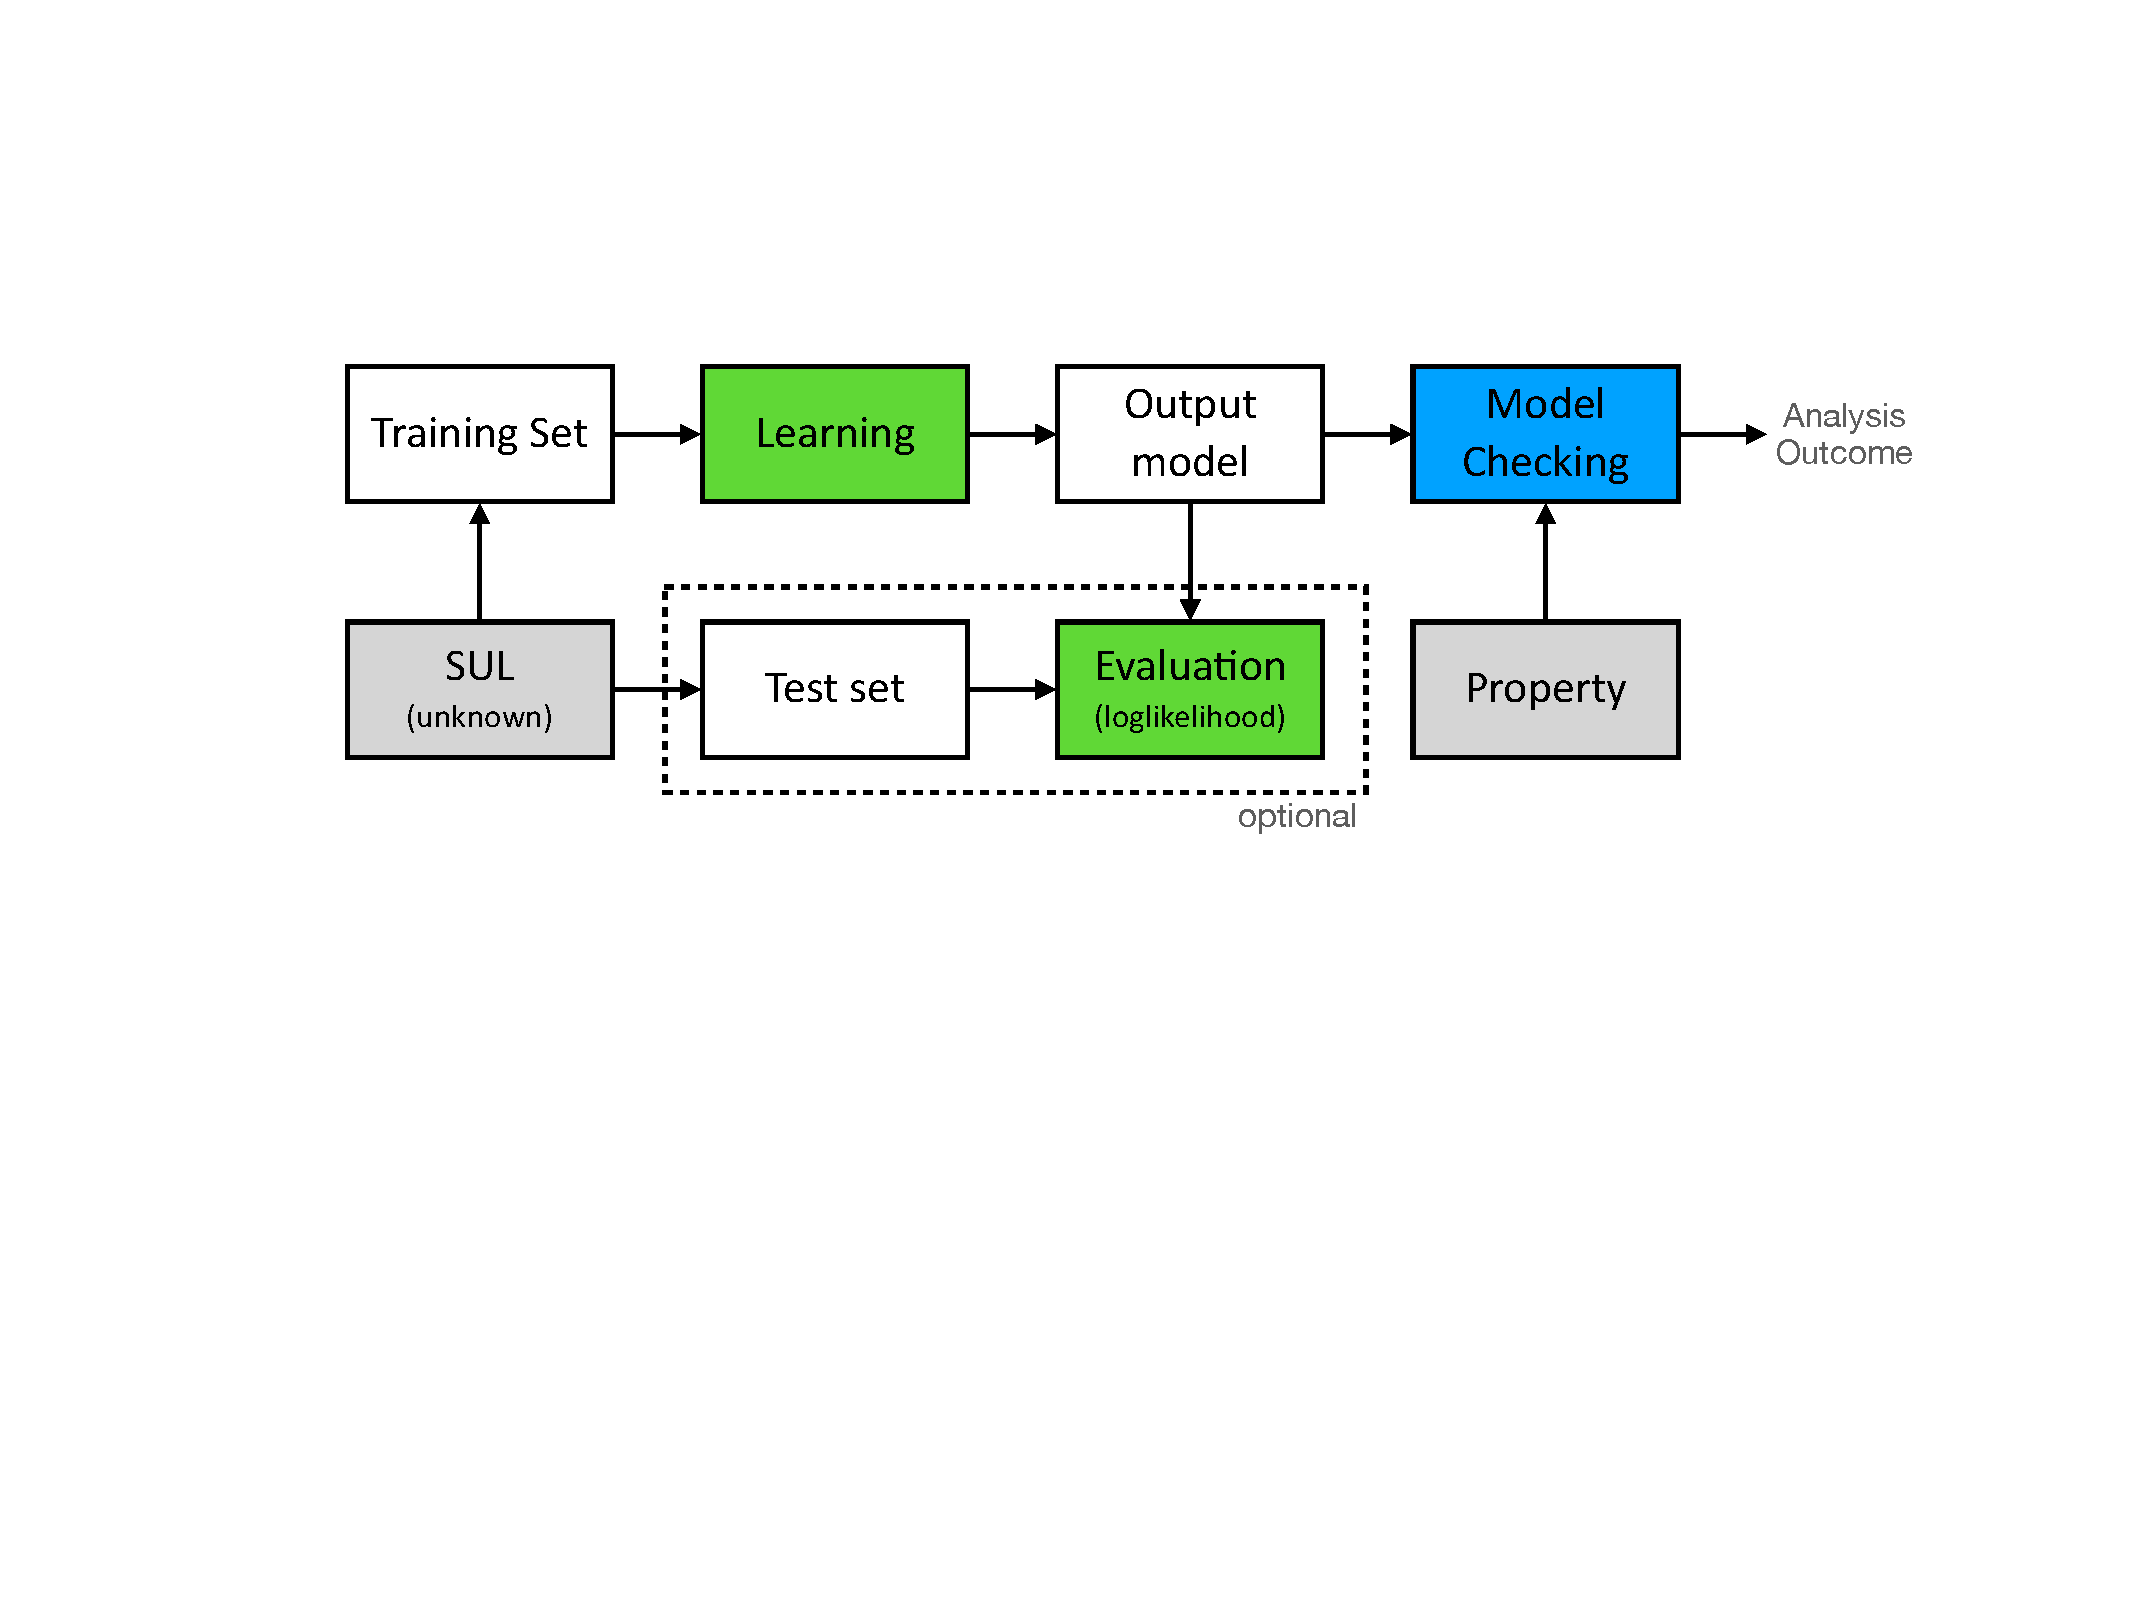
\includegraphics[width=\columnwidth]{figures/workflow.pdf}
    \caption{Modeling and verification workflow using \Jajapy. Phases involving \Jajapy\ are highlighted in green, while the blue phase represents verification using \Storm~or \Prism.}
    \label{fig:workflow}
\end{figure}


In this context, we refer to the \textit{training set} as the collection of observation traces used to infer a model of the SUL, and the \textit{test set} as a separate set of traces used to evaluate the quality of the learned model.

\Jajapy\ supports learning various types of models, depending on the structure of the training data.
For clarity, this paper focuses specifically on the new features introduced in \JajapyTwo, which primarily target Markov chains.
However, these improvements are equally applicable to other classes of Markov models supported by the tool.

At the core of \Jajapy's learning capabilities are several variants of the Baum-Welch (BW) algorithm~\cite{Baum70,Rabiner89}, adapted for discrete-time Markov chains (MCs), Markov decision processes (MDPs)\cite{BacciILR21}, and continuous-time Markov chains (CTMCs)\cite{BacciILR23}.

Each algorithm requires two inputs: a training set and the desired number of states for the output model.
The process begins with the creation of a randomly initialized model (e.g., a Markov chain) and iteratively updates its transition probabilities, increasing the likelihood of transitions that better explain the observed traces.

The efficiency and accuracy of the learning process depends heavily on the choice of the initial hypothesis.
To improve convergence and model quality, \Jajapy\ allows users to supply a custom initial hypotheses in several formats, including \Stormpy~sparse models, \Prism-files, or native \Jajapy\ model definitions.

An example of using \Jajapy\ to learn a 10-state Markov chain from a training set, starting from a random initial hypothesis, is shown in \autoref{fig:run-bw}.


\begin{listing}[htb!]
    \begin{minted}{python} 
    import jajapy
    training_set = jajapy.loadSet("Path/to/data")
    type(training_set) # list 

    learned_model = jajapy.BW().fit(training_set, nb_states=10)
    type(learned_model) # stormpy.SparseDtmc 
    \end{minted}
    \caption{Example of using \Jajapy's BW implementation to learn a 10-state Markov chain from a training set.}
    \label{fig:run-bw}
\end{listing}


\Jajapy\ supports reading \Prism\ files, using \Storm\ (through \Stormpy), as well as direct verification of learned model, through properties, provided the properties are supported.
Alternatively, the model can be exported to \Prism's format for verification using the \Prism\ model checker.


\subsection{CuPAAL}\label{subsec:cupaal}
\Cupaal is a tool developed in C++ that extends the work done in \Jajapy\ by implementing the Baum-Welch algorithm with an \gls{add}-based approach instead of a recursive method.
The goal of \Cupaal\ is to leverage \glspl{add} to improve the efficiency of learning Markov models, particularly in large-scale applications where traditional recursive methods may become computationally expensive.

\Cupaal\ has undergone multiple iterations.
Initially, it implemented a partial \gls{add}-based approach, where only the calculation of the alpha and beta values of the Baum-Welch algorithm were implemented using \glspl{add}.
This partial implementation served as an initial proof-of-concept to determine whether incorporating \glspl{add} could yield performance benefits compared to the recursive approach employed by \Jajapy.

Following promising results from the partial implementation, further development led to a fully \gls{add}-based version of \Cupaal\ for \glspl{hmm}.
This iteration replaced all recursive computations with \glspl{add}, enabling more efficient execution, particularly for large models.
The transition to a fully \gls{add}-based approach demonstrated the potential for significant computational savings and scalability improvements, reinforcing the viability of this method for broader applications beyond our initial research scope.

Because there is no notion of \gls{hmm} in the \Prism\ formalism, we've implemented the \gls{bw} algorithm for use with \glspl{mc}.
Given the similarities between these model types, we've reused a lot of the previous work in the implementation.

By building upon \Jajapy\ and developing \Cupaal, we have been able to evaluate the impact of using \glspl{add} in probabilistic model learning.
